\chapter{Deep learning 1}
\begin{introduction}[keywords]
    \item Feature extraction : 特征提取
    \item Logistic Regression : 逻辑回归
    \item Heuristic model : 启发式模型
    \item Maximum Likelihood Estimation : 最大似然估计
    \item Stochastic Gradient Descent : 随机梯度下降
    \item Multilayer Perceptron : 多层感知机
    \item Dense layer : 全连接层
\end{introduction}

\begin{note}
    从本章开始的几章内容和 AI 基础课程高度重合,如果你对其中的内容有所疑问,亦可参考笔者的 AI 基础课程笔记:\href{https://arthals.ink/tags/ai\%20\%E5\%9F\%BA\%E7\%A1\%80}{Blog} / \href{https://github.com/zhuozhiyongde/Fundamentals-of-Artificial-Intelligence-2024Spring-PKU/tree/main/Note}{GitHub Repo}
\end{note}

\section{Feature Description}

\begin{problem}
    我们已经知道了如何去 detect 一些点,下一步如何通过描述他们进行匹配呢?
\end{problem}

    将图像内容转换为不受平移、旋转、缩放和其他成像参数影响的局部特征坐标。例如,房子的地点,大小,风格,建造时间,当前状况等。基于这些 features, 我们有:
    \begin{itemize}
        \item Heuristic model (启发式模型): $y = (10-\text{location})\times \text{area}$
        \item Parametric model (参数模型): $y = \phi_\theta(F)$
    \end{itemize}
\begin{note}
拥有一些 observations 后,我们就可以 fit $\theta$.
\end{note}

\section{Machine learning}

当我们有了一组 observations $\{(x_i, y_i)\}_{i=1}^N$, 我们希望找到 $y$ 和 $x$ 的关系。
\begin{itemize}
    \item Line fitting: 我们知道这个关系近似为线性关系,所以用 $y = mx + b$ 来拟合(先验知识)。
    \item Training neural network: 我们用参数模型来拟合,但是我们对其所知甚少,这和直线拟合没有本质区别。
\end{itemize}
\begin{definition}[Outline]
    \begin{itemize}
        \item 设立任务
        \item 准备数据 $\to$ 需要标注好的数据(labeled dataset)
        \item 建立模型 $\to$ 构造神经网络
        \item 决定目标 $\to$ 损失函数
        \item 进行拟合 $\to$ 训练
        \item 测试 $\to$ 评估在测试数据上的表现
    \end{itemize}
\end{definition}

\subsection{Task}
\begin{figure}[htbp]
    \centering
    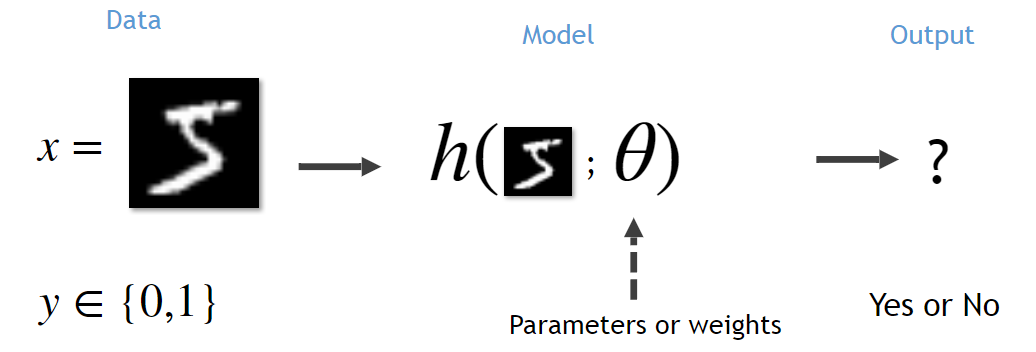
\includegraphics[width=0.6\textwidth]{figures/ministdataset.png}
    \caption{pipeline}
    \label{fig:ml-pipeline}
\end{figure}

给定一张图片,以参数 $\theta$(称作参数 parameters 或者权重 weights)构建一个模型,输出这张图片是否为 5(输出为 0/1,即是/不是)。

实际上我们输出一个是 5 的概率,我们显然希望对于 5 的图片,输出接近 1,对于不是 5 的图片,输出接近 0。

\subsection{Data}

\begin{figure}[H]
    \centering
    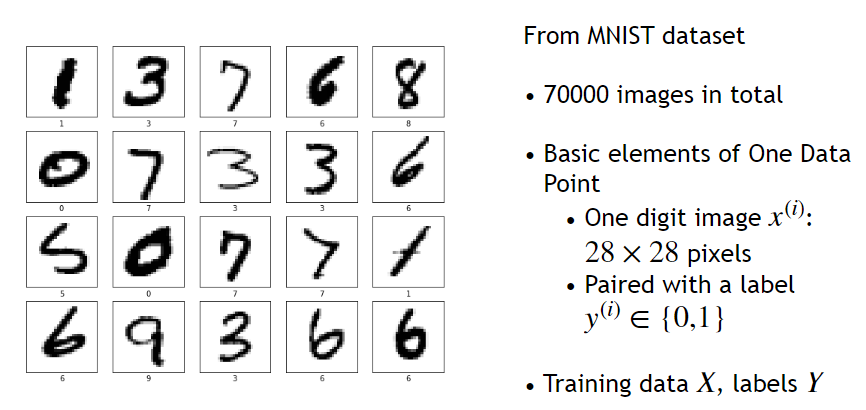
\includegraphics[width=0.8\textwidth]{figures/Mnistdataset.png}
    \caption{MINIST Dataset}
    \label{fig:ml-dataset}
\end{figure}

\subsection{Model}
我们使用所谓逻辑回归 (Logistic Regression) 来进行分类,其模型为:
$$h(x) = g(\theta^T x) = \frac{1}{1 + e^{-\theta^T x}}$$

\begin{figure}[htbp]
    \centering
    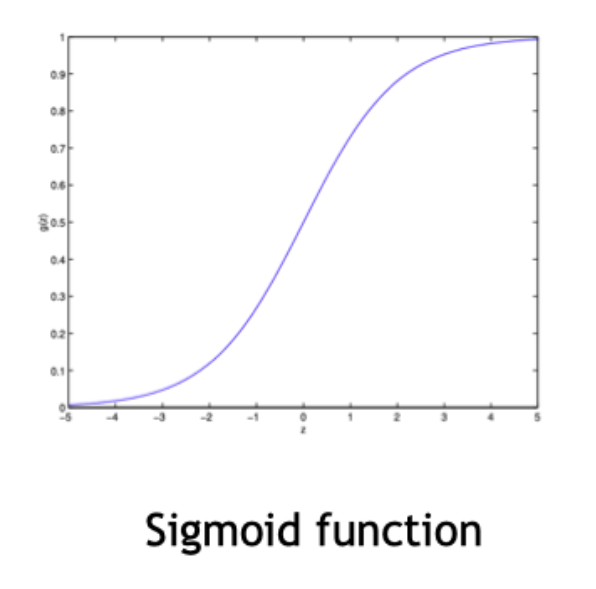
\includegraphics[width=0.4\textwidth]{figures/sigmoid.png}
    \caption{sigmoid function}
    \label{fig:sigmoid}
\end{figure}

\begin{note}
    这里的 $g$ 是 sigmoid 函数 $g(z) = \frac{1}{1 + e^{-z}}$, 将 $z\in \mathbb{R}$ 映射到 $[0, 1]$, 提供非线性。
\end{note}
\subsection{Loss function}
\begin{definition}[最大似然估计]
    \begin{itemize}
        \item 即最大化似然函数,使得在假定的统计模型下,观察到的数据是最有可能的。
        \item 参数空间中最大化似然函数的点 (实际上是网络权重) 称为最大似然估计。
    \end{itemize}
\end{definition}
回到原任务 (分类一张图片是否是 5),首先定义符号:

\begin{itemize}
    \item 输入数据 $X = \{x^{(1)}, x^{(2)}, ..., x^{(N)}\}$,其中 $x^{(i)} \in \mathbb{R}^{28 \times 28}$ 是第 $i$ 个图像  
    \item 标签 $Y = \{y^{(1)}, y^{(2)}, ..., y^{(N)}\}$,其中 $y^{(i)} \in \{0,1\}$ 表示图像 $x^{(i)}$ 是否属于类别 5  
    \item 参数 $\theta$,以之为参数的模型 $h_\theta(x^{(i)}) \in [0,1]$ 输出图像 $x^{(i)}$ 为类别 5 的概率  
\end{itemize}

对于单个样本的条件概率(给定 $\theta$ 和输入 $x^{(i)}$ 的情况下,模型正确输出 $y^{(i)}$ 的概率):  
$$
p(y^{(i)} | x^{(i)}, \theta) = h_\theta(x^{(i)})^{y^{(i)}} \cdot \left(1 - h_\theta(x^{(i)})\right)^{1 - y^{(i)}}
$$


\begin{note}
    这里 $y^{(i)}$ 取值为 0 或 1, $x^{(i)}$ 是 28 $\times$ 28 的图像,$\theta$ 是我们要学习的参数,$h_\theta(x^{(i)})$ 是模型认为 $x^{(i)}$ 是 5 的概率。

    由于 $y^{(i)}$ 是标签,所以 $y^{(i)}$ 和 $1-y^{(i)}$ 有一个取值为 0 另一个为 1,这被用于选择正确的损失项,当真实标签 $y^{(i)}=1$ 时,$h_\theta(x^{(i)})$ 项用于计算我们标注正确的概率;当 $y^{(i)}=0$ 时,$(1 - h_\theta(x^{(i)}))$ 项用于计算我们标注正确的概率。
\end{note}
自然地假设所有数据点独立同分布,因此我们有:
$$ p(Y|X, \theta) = \prod_{i=1}^N p(y^{(i)}|x^{(i)}, \theta) = \prod_{i=1}^N h_{\theta}(x^{(i)})^{y^{(i)}} (1 - h_{\theta}(x^{(i)}))^{1-y^{(i)}} $$

Loss 就是我们想去最小化的东西,这里可以有所谓 Negative Log Likelihood (NLL) loss :
$$ \mathcal{L}({\theta}) = -\log p(Y|X, \theta) = -\sum_{i=1}^N \left( y^{(i)} \log h_{\theta}(x^{(i)}) + (1 - y^{(i)}) \log (1 - h_{\theta}(x^{(i)})) \right) $$

\subsection{Training : Gradient Descent}
此时我们可以去定义一个优化问题,但通用的优化问题是困难的,有一些问题类型可以被有效地解决,例如:
\begin{itemize}
    \item Convex optimization: 目标函数是一个凸函数,约束条件是一个凸集。
    \item Linear programming: 目标函数是线性的,约束条件是线性的。
    \item Least squares: 目标函数是二次函数,约束条件是线性的。
\end{itemize}
如果我们将参数空间放到横轴,Loss 放到纵轴,我们可以自然地得到一个曲面 (这是 Loss 具备的数学性质), 对于曲面自然存在凸性的局部或者整体:

% 将 loss1.png 和 loss2.png 左右排布放在一起,高度对齐

\begin{figure}[htbp] 
        \centering
        \begin{minipage}[b]{0.4\linewidth}
            \centering
            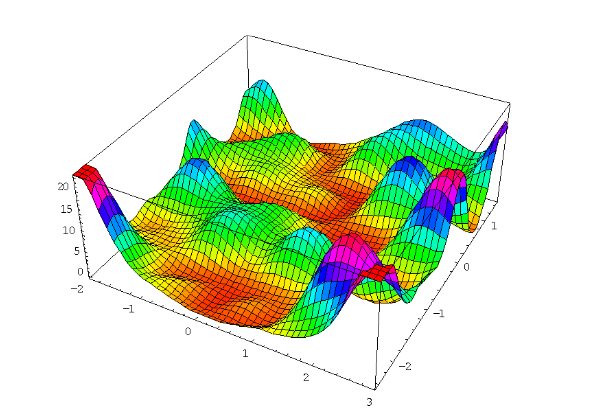
\includegraphics[width=\textwidth]{figures/loss1.png}
            \caption{Non-convex energy landscape}
            \label{fig:loss1}
        \end{minipage}
        \hfill
        \begin{minipage}[b]{0.2\linewidth}
            \centering
            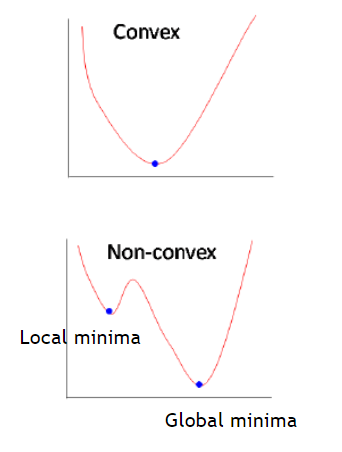
\includegraphics[width=\textwidth]{figures/loss2.png}
            \caption{minima}
            \label{fig:loss2}
        \end{minipage}
\end{figure}

\begin{definition}[Gradient Descent]
    \begin{itemize}
        \item 每次迭代的公式 :
        $$\theta_{t+1} = \theta_t - \alpha \nabla_{\theta} \mathcal{L}(\theta_t)$$
        \item 其中 $\alpha$ 是学习率,$\nabla_{\theta} \mathcal{L}(\theta_t)$ 是 Loss 的梯度。
    \end{itemize}
\end{definition}

Sigmoid 函数通常定义为:

$$
\sigma(x) = \frac{1}{1 + e^{-x}}
$$

为了推导它的导数,我们首先对其进行变形。

$$
\begin{aligned}
(1 + e^{-x})·\sigma(x) &= 1\\
e^{-x}·(-1)·\sigma(x) + \sigma'(x)·(1 + e^{-x}) &=0\\
\sigma'(x)·(1 + e^{-x}) &= e^{-x}·\sigma(x)\\
\sigma'(x)&=(1-\sigma(x))·\sigma(x)
\end{aligned}
$$

最终,我们得到了 sigmoid 函数的导数:

$$
\sigma'(x) = (1-\sigma(x))\sigma(x)
$$

\begin{note}
而对于我们的 NLL loss, 令 $h_\theta(x) = g(\theta^T x)$,注意到 sigmoid 函数有 $g'(z) = g(z)(1-g(z))$, 我们可以得到 :
$$\begin{aligned}\frac{\partial\mathcal{L}}{\partial\theta_{j}}&=-\sum\left(y\frac1{g(\theta^Tx)}-(1-y)\frac1{1-g(\theta^Tx)}\right)\frac\partial{\partial\theta_j}g(\theta^Tx)\\&=-\sum\left(y\frac1{g(\theta^Tx)}-(1-y)\frac1{1-g(\theta^Tx)}\right)g(\theta^Tx)(1-g(\theta^Tx))\frac\partial{\partial\theta_j}\theta^Tx\\&=-\sum\left(y(1-g(\theta^Tx))-(1-y)g(\theta^Tx)\right)x_j\\&=-\sum\left(y-h_\theta(x)\right)x_j\end{aligned}
$$
\end{note}
\begin{theorem}[Stochastic Gradient Descent]
    所谓的 Batch Gradient Descent 是指每次迭代都使用所有的训练数据来计算梯度,但是这样会非常慢,因此我们可以使用 Stochastic Gradient Descent (SGD), 每次迭代只使用随机出的 N 对样本。此时令:
    $$\nabla_{\theta} \mathcal{L}(\theta_t) = \frac{1}{N}\sum_{i=1}^N \nabla_{\theta} \mathcal{L}(\theta_t, x_i, y_i)$$
    此外,SGD 有助于跳出 local minima, 但是会导致 loss 函数震荡。
\end{theorem}

\subsection{Testing}
训练后,我们需要测试泛化性,也就是模型在未见过的数据上的表现。

\section{Multilayer Perceptron}

\begin{figure}[htbp]
    \centering
    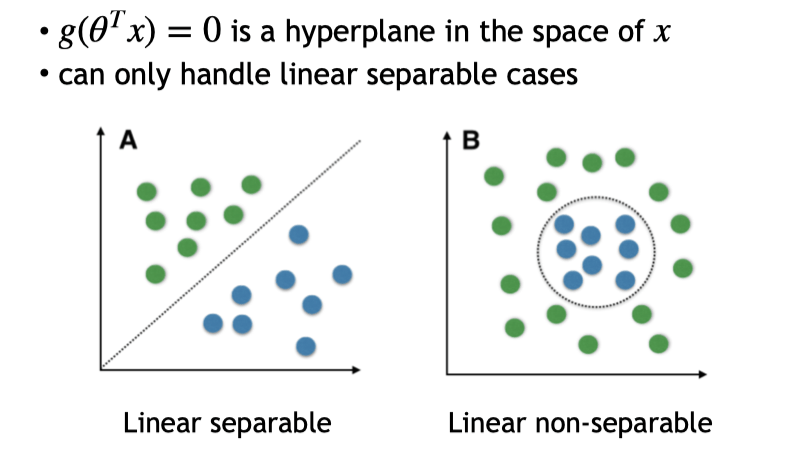
\includegraphics[width=0.8\textwidth]{figures/single_layer_issue.png}
    \caption{单层网络解决不了线性不可分问题}
    \label{fig:single-layer-issue}
\end{figure}



\begin{note}
    单层网络解决不了线性不可分的问题,因此我们需要 MLP. 
\end{note}


$$ f(x; \theta) = g(W_2(g(W_1 x + b_1)) + b_2) $$


\begin{figure}[htbp]
    \centering
    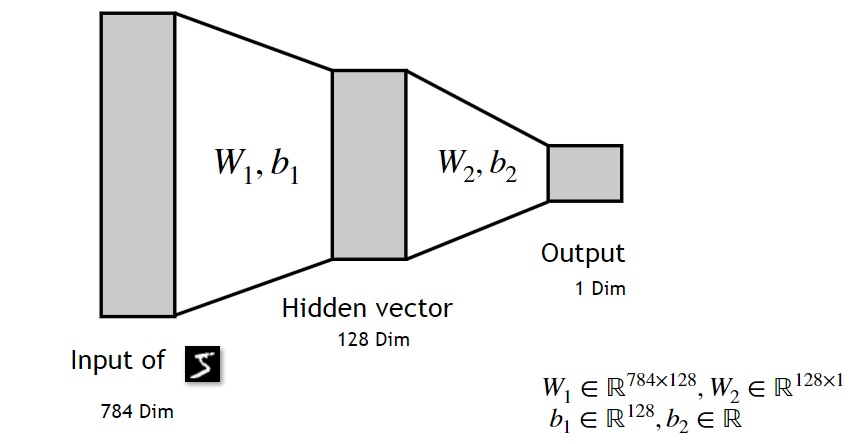
\includegraphics[width=0.8\textwidth]{figures/mlp.png}
    \caption{MLP 前向过程示例}
    \label{fig:mlp}
\end{figure}


\subsection{Chain Rule}
\begin{problem}
    如何训练 MLP? 如何获取梯度?
\end{problem}
使用矩阵计算链式法则的结果解决这个问题,得到每个参数 $W_i, b_i$ 的梯度,那就可以更新参数了。我们判断一个网络是否可以更新,一个直观的标准就是看他的前向过程是否可微可导。即便实际操作未必参与计算。
\begin{figure}[htbp]
    \centering
    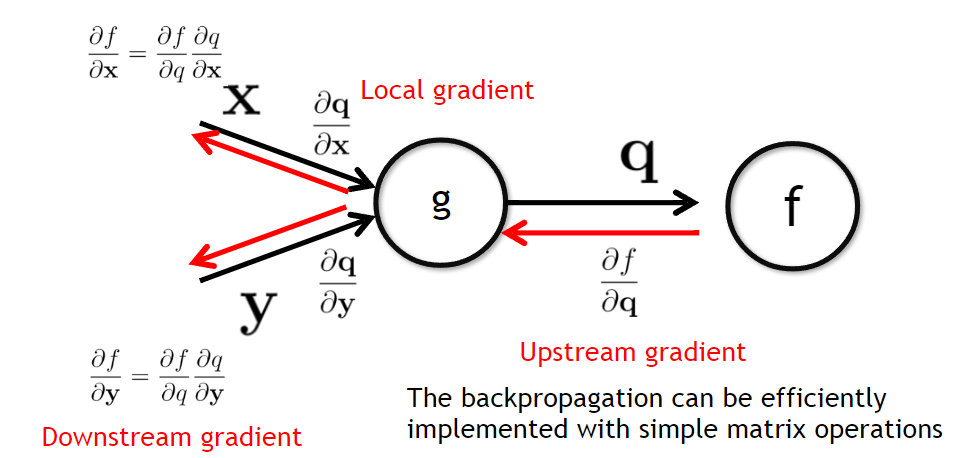
\includegraphics[width=0.8\textwidth]{figures/chainrule.png}
    \caption{链式法则求梯度}
    \label{fig:chainrule}
\end{figure}

\clearpage

\subsection{Activation function}

\begin{figure}[htbp]
    \centering
    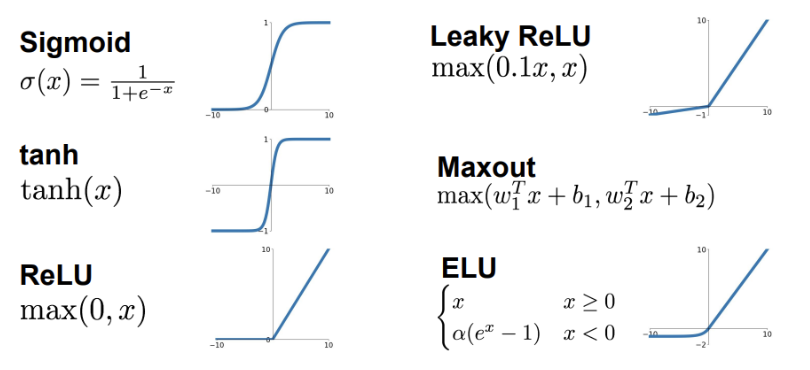
\includegraphics[width=0.8\textwidth]{figures/activationfunc.png}
    \caption{常用激活函数}
    \label{fig:activation-func}
\end{figure}

\begin{note}
激活函数替代我们的 $g$, 其中 ReLU 通常是大部分问题的默认选择
\end{note}

\begin{definition}[Fully connected layer]
    \begin{itemize}
        \item 每个神经元都和前一层的每个神经元相连,也叫做 Dense layer.
    \end{itemize}
\end{definition}

\subsection{Problems of MLP}
视觉信号过程中,MLP 可能会遇到一些问题:
\begin{itemize}
    \item 计算量大,将高分辨率图像向量化非常耗时。
    \item 扁平化操作会破坏图像的局部结构。
\end{itemize}